\documentclass[aima203_lecturenotes_ku.tex]{subfiles}

\setcounter{chapter}{3}
\begin{document}
\chapter{Interpolation}
\section{Introduction}
The central problem of numerical analysis is: given a set of tabular values \\
$(x_0,y_0), (x_1,y_1),(x_2,y_2),...,(x_n,y_n)$ satisfying the realtion $y=f(x)$, where the explict nature of $f(x)$ is not known, is to find a simpler function $\phi (x)$ such that $\phi (x)$ and $f(x)$ agree at the set of the tabulated points. Such process is called \textbf{interpolation}. If $\phi (x)$ is a polynomial, then the process is called \textit{polynomial interpolation}, and $\phi (x)$ a interpolating polynomial. In this chapter we are concerned with only polynomial interpolation.

\begin{theorem}[Weiestrass Theorem]
If $f(x)$ is continuous in $x_0 \geq x \geq x_n$, then given $\epsilon >0$, there exists a polynomial $P(x)$ such that $|f(x)-P(x)| < \epsilon$, for all $x \in (x_0, x_n)$.
\end{theorem}
So, this gives the justification for approximating a function with a polynomial function.

\section{Finite Differences}
Assume that we have a table of values $(x_i,y_i), \; i=0,1,\, ..., \, n$ of any function $y=f(x)$. Suppose the values of $x$ are equally spaced, i.e., $x_i=x_0 + ih, \; i=0,1,\, ..., \, n$ for some constant $h$. \\
Then, the values $y_1 - y_0, \, y_2 - y_1, \, ..., \, y_n - y_{n-1}$, are called the differences of $y$. If $y_{i+1} - y_i$ is taken as the $i^{th}$ difference, then we are considering it as a forward difference, if it is taken as the $(i+1)^{th}$ differnce then, we are considering it as a backward differnce, and if it is taken as $((i+1)/2)^{th}$ then, we are considering it as a central differnce. More on these topics in coming subsections.

\subsection{Forward Differences}
The forward differnce $\Delta y_i$ is defined as $\Delta y_i = y_{i+1} - y_i$, where $\Delta$ is called the \textit{forward difference operator}. We have,
\begin{equation}
  \label{forward}
  \Delta y_0 = y_1 - y_0, \hspace{5mm} \Delta y_1 = y_2 - y_1, \hspace{5mm} ..., \hspace{5mm} \Delta y_{n-1} = y_{n} - y_{n-1}
\end{equation}
These differnces $\Delta y_i, \; i=0,1,\, ..., \, (n-1)$ are called \textit{first forward differences}.
\begin{itemize}
\item For $(n+1)$ points, there are $n$ forward differnces.
\item These $n$-forward differnces begin at $\Delta y_0$, and end at $\Delta y_{n-1}$. There is no $\Delta y_n$.
\end{itemize}

\subsubsection{Second Forward Differnces}
The forward differences of the first forward differences are called second forward differences. They are denoted by $\Delta ^2 y_i, \; i=0,1,\, ..., \, (n-2)$. That is,
\begin{equation}
  \label{forward2}
  \Delta ^2 y_0 = \Delta y_1 - \Delta y_0, \hspace{5mm} \Delta ^2 y_1 = \Delta y_2 - \Delta y_1, \hspace{5mm} ..., \hspace{5mm} \Delta ^2 y_{n-2} = \Delta y_{n} - \Delta y_{n-1}
\end{equation}
Here, $\Delta ^2 y_0 = \Delta y_1 - \Delta y_0 = y_2 - y_1 - (y_1 - y_0) = y_2 -2y_1 - y_0$.

\subsubsection{Higer Order Forward Differnces}
Here, $\Delta ^3 y_0 = \Delta ^2 y_1 - \Delta ^2 y_0 = \Delta y_2 - \Delta y_1-(\Delta y_1 - \Delta y_0) = ... = y_3 - 3y_2 + 3y_1- y_0$. \\
The coefficients occuring are the \textbf{binomial coefficients}.

\subsubsection{Programming}
For practical computations, the following notation is useful: $y_j=DEL(0,j)$, and
\begin{gather*}
  \Delta y_j = DEL(0,j+1) - DEL(0,j) \\
  \Delta ^i y_j = DEL(i-1,j+1) - DEL(i,j)
\end{gather*}

\subsection{Backward Differences}
The backward differnce $\nabla y_{i+1}$ is defined as $\nabla y_{i+1} = y_{i+1} - y_i$, where $\nabla$ is called the \textit{backward difference operator}. We have,
\begin{equation}
  \label{backward}
  \nabla y_1 = y_1 - y_0, \hspace{5mm} \nabla y_2 = y_2 - y_1, \hspace{5mm} ..., \hspace{5mm} \nabla y_n = y_{n} - y_{n-1}
\end{equation}
These differnces $\nabla y_{i+1}, \; i=0,1,\, ..., \, (n-1)$ are called \textit{first backward differences}.

\begin{itemize}
\item For $(n+1)$ points, there are $n$ backward differnces.
\item These $n$-backward differnces begin at $\nabla y_1$, and end at $\nabla y_n$. There is no $\nabla y_0$.
\end{itemize}

\subsubsection{Second Backward Differnces}
The backward differences of the first backward differences are called second backward differences. They are denoted by $\nabla ^2 y_{i+2}, \; i=0,1,\, ..., \, (n-2)$. That is,
\begin{equation}
  \label{backward2}
  \nabla ^2 y_2 = \nabla y_2 - \nabla y_1, \hspace{5mm} \nabla ^2 y_3 = \nabla y_3 - \nabla y_2, \hspace{5mm} ..., \hspace{5mm} \nabla ^2 y_n = \nabla y_n - \nabla y_{n-1}
\end{equation}
Here, $\nabla ^2 y_2 = \nabla y_2 - \nabla y_1 = y_2 - y_1 - (y_1 - y_0) = y_2 -2y_1 - y_0$.

\subsubsection{Higer Order Backward Differnces}
Here, $\nabla ^3 y_3 = \nabla ^2 y_3 - \nabla ^2 y_2 = \nabla y_3 - \nabla y_2-(\nabla y_2 - \nabla y_1) = ... = y_3 - 3y_2 + 3y_1- y_0$. \\
The coefficients occuring are the \textbf{binomial coefficients}.

\subsection{Central Differences}
The central differnce $\delta y_{i+1/2}$ is defined as $\delta y_{i+1/2} = y_{i+1} - y_i$, where $\delta$ is called the \textit{central difference operator}. We have,
\begin{equation}
  \label{central}
  \delta y_{1/2} = y_1 - y_0, \hspace{5mm} \delta y_{3/2} = y_2 - y_1, \hspace{5mm} ..., \hspace{5mm} \delta y_{(2n-1)/2} = y_{n} - y_{n-1}
\end{equation}
These differnces $\delta y_{i+1/2}, \; i=0,1,\, ..., \, (n-1)$ are called \textit{first central differences}.
\begin{itemize}
\item For $(n+1)$ points, there are $n$ first central differnces.
\item These $n$-central first differnces begin at $\delta y_{1/2}$, and end at $\delta y_{(2n-1)/2}$.
\end{itemize}

\subsubsection{Second Central Differnces}
The central differences of the first central differences are called second central differences. They are denoted by $\delta ^2 y_{i}, \; i=1,\, ..., \, (n-1)$ $\delta^2 y_{i} = \delta y_{i+1/2} - \delta y_{(i-1) + 1/2}$. That is,
\begin{equation}
  \label{central2}
  \delta ^2 y_1 = \delta y_{3/2} - \delta y_{1/2}, \hspace{5mm} \delta ^2 y_2 = \delta y_{5/2} - \delta y_{3/2}, \hspace{5mm} ..., \hspace{5mm} \delta ^2 y_{n-1} = \delta y_{(2n-1)/2} - \delta y_{(2n-3)/2}
\end{equation}
Here, $\delta ^2 y_1 = \delta y_{3/2} - \delta y_{1/2} = y_2 - y_1 - (y_1 - y_0) = y_2 -2y_1 - y_0$.

\subsubsection{Higer Order Central Differnces}
Here, $\delta ^3 y_{3/2} = \delta ^2 y_2 - \delta ^2 y_1 = \delta y_{5/2} - \delta y_{3/2}-(\delta y_{3/2} - \delta y_{1/2}) = ... = y_3 - 3y_2 + 3y_1- y_0$.

\subsection{Equivallency of the differences}
From the above subsections we can see that, the same numbers occurs at the same positions whether we use forward backward or central differences. That is, $$\Delta y_0 = \nabla y_1 = \delta y_{1/2}, \hspace{2cm} \Delta^2 y_0 = \nabla ^2 y_1 = \delta ^2 y_1, \hspace{1cm} \Delta ^3 y_0 = \nabla ^3 y_3 = \delta ^3 y_{3/2} $$

\section{Newton's formula for Interpolation}
Given $(n+1)$ points, $(x_0,y_0), \, (x_1,y_1), \, ..., \, (x_n,y_n)$ of $x$ and $y(x)$, with $x$ values equally spaced, we find a polynomial $y_n(x)$ of $n$th degree such that, $y(x)$ and $y_n(x)$ agree at the given points. \\
If we consider $y_n(x)$ to be the polynomial:
\begin{equation}
  \begin{gathered}
  y_nx(x)= a_0 +a_1(x-x_0) +a_2(x-x_0)(x-x_1)+a_3(x-x_0)(x-x_1)(x-x_2) \\[1mm]
  + ... + a_n(x-x_0)(x-x_1)...(x-x_{n-1}).
  \end{gathered}
\end{equation}
\vspace{2mm}
Then, $\displaystyle a_0 = y_0, \;\; a_1=\frac{y-y_1}{x_1-x_0}=\frac{\Delta y_0}{h}, \;\; a_2 = \frac{\Delta ^2 y_0}{2!\, h^2}, \;\; a_3 = \frac{\Delta ^3 y_0}{3!\, h^3}, \;..., \;  a_n = \frac{\Delta ^n y_0}{n!\, h^n} $ \\[1mm]
where, $h$ is the $x_i - x_j, \;\;\; i \neq j$. \\
Setting $x=x_0 +ph$, we get,
\begin{equation}
  \label{newtforward}
 \begin{gathered}
  y_n(x) = y_0 + p \Delta y_0 + \frac{p(p-1)}{2!}\, \Delta ^2 y_0 + \frac{p(p-1)(p-2)}{3!}\, \Delta ^3 y_0 + ... \\[1mm]
  + \frac{p(p-1)(p-2)...(p-(n-1))}{n!}\, \Delta ^n y_0
\end{gathered}
\end{equation}
This formula~\ref{newtforward} is the \textbf{Newton's forward difference interpolation} formula.

\subsection{Newton's backward difference Interpolation}
If we consider $y_n(x)$ to be the polynomial:
\begin{equation}
  \begin{gathered}
  y_nx(x)= a_0 +a_1(x-x_n) +a_2(x-x_n)(x-x_{n-1})+a_3(x-x_n)(x-x_{n-1})(x-x_{n-2}) \\[1mm]
  + ... + a_n(x-x_n)(x-x_{n-1})(x-x_{n-2})...(x-x_1).
  \end{gathered}
\end{equation}
Then we get the following formula for $y_n(x)$.
\begin{equation}
  \label{newtbackward}
 \begin{gathered}
  y_n(x) = y_n + p \nabla y_n + \frac{p(p-1)}{2!}\, \nabla ^2 y_n + \frac{p(p-1)(p-2)}{3!}\, \nabla ^3 y_n + ... \\[1mm]
  + \frac{p(p-1)(p-2)...(p-(n-1))}{n!}\, \nabla ^n y_n
\end{gathered}
\end{equation}
This formula~\ref{newtbackward} is the \textbf{Newton's backward difference interpolation} formula.

\begin{remark}
The Newton's forward difference interpolation formula is useful for interpolating near the begining of the tabular values and the Newton's backward difference interpolation formula is useful for interpolating near the end of the tabular values.
\end{remark}

\begin{figure}[h]
  \centering
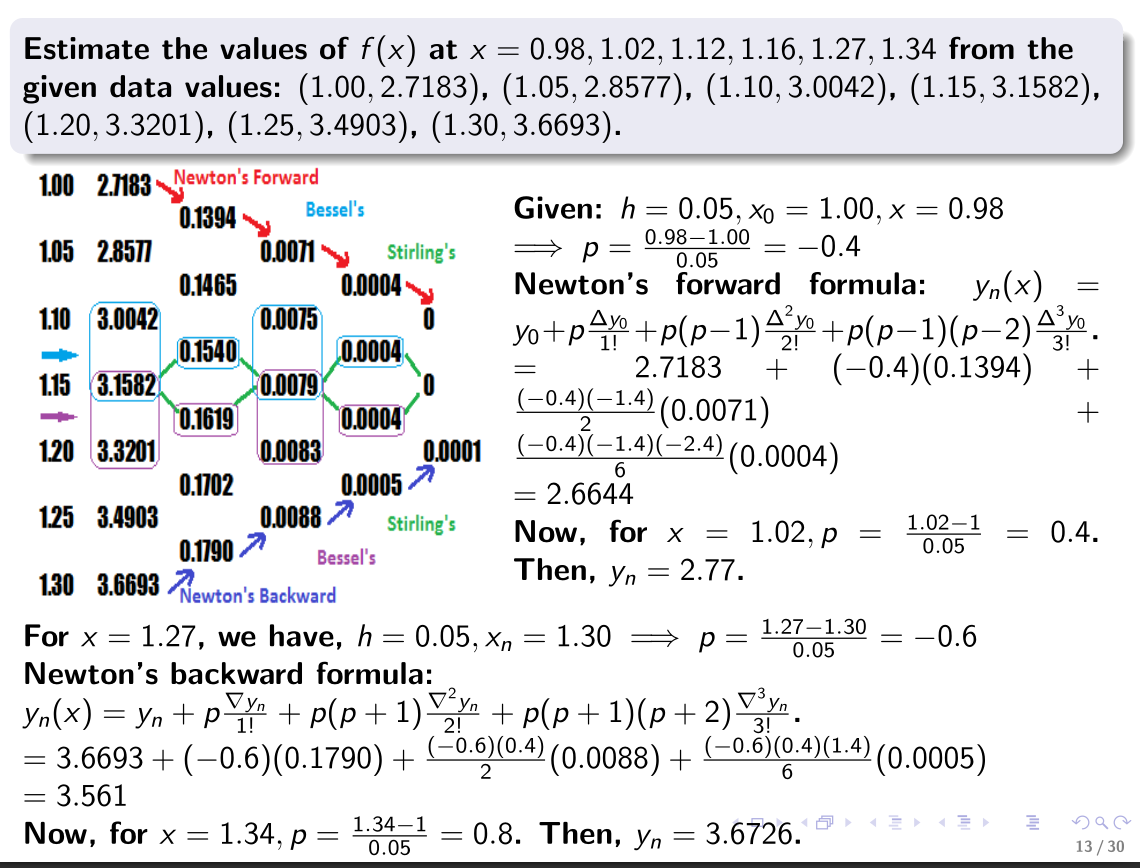
\includegraphics[width=13cm, height=11cm]{newt_forward.png}
\end{figure}


\begin{enumerate}
\item Find the cubic polynomial which takes the following values: $y(1)=24, \;\;\;  y(3)=120,  \;\;\; y(5)=336,  \;\;\; y(7)=720$. Then obtain the value of $y(8)$.
\item Find a cubic polynomial which fits the data: $(-2, -12)  \;\;\; (-1, -8),  \;\;\; (2,3),  \;\;\; (3,5)$.
\end{enumerate}
\section{Interpolation with Unevenly spaced points}
This section discusses the inerpolation method for unequally spaced values of the argument.

\subsection{Lagrange's Interpolation Formula}
Let $y(x)$ be continuous and differentiable $(n+1)$ times in the interval $(a,b)$. Given $(n+1)$ points, $(x_0,y_0), \, (x_1,y_1), \, ..., \, (x_n,y_n)$ of $x$ and $y(x)$, where $x$ values not necessarily equally spaced, we find a polynomial $L_n(x)$ of $n$th degree such that, $y(x)$ and $L_n(x)$ agree at the given points. \\
The formula $\sum_{i=0}^n \; l_i(x)\, y_i$, where $\displaystyle l_i(x) = \frac{(x-x_0)(x-x_1)...(x-x_{i-1})(x-x_{i+1})...(x-x_n)}{(x_i-x_0)(x_i-x_1)...(x_i-x_{i-1})(x_i-x_{i+1})...(x_i-x_n)} $ \\[2mm]  is called the Lagrange's Interpolating formula.

\begin{figure}[h]
  \centering
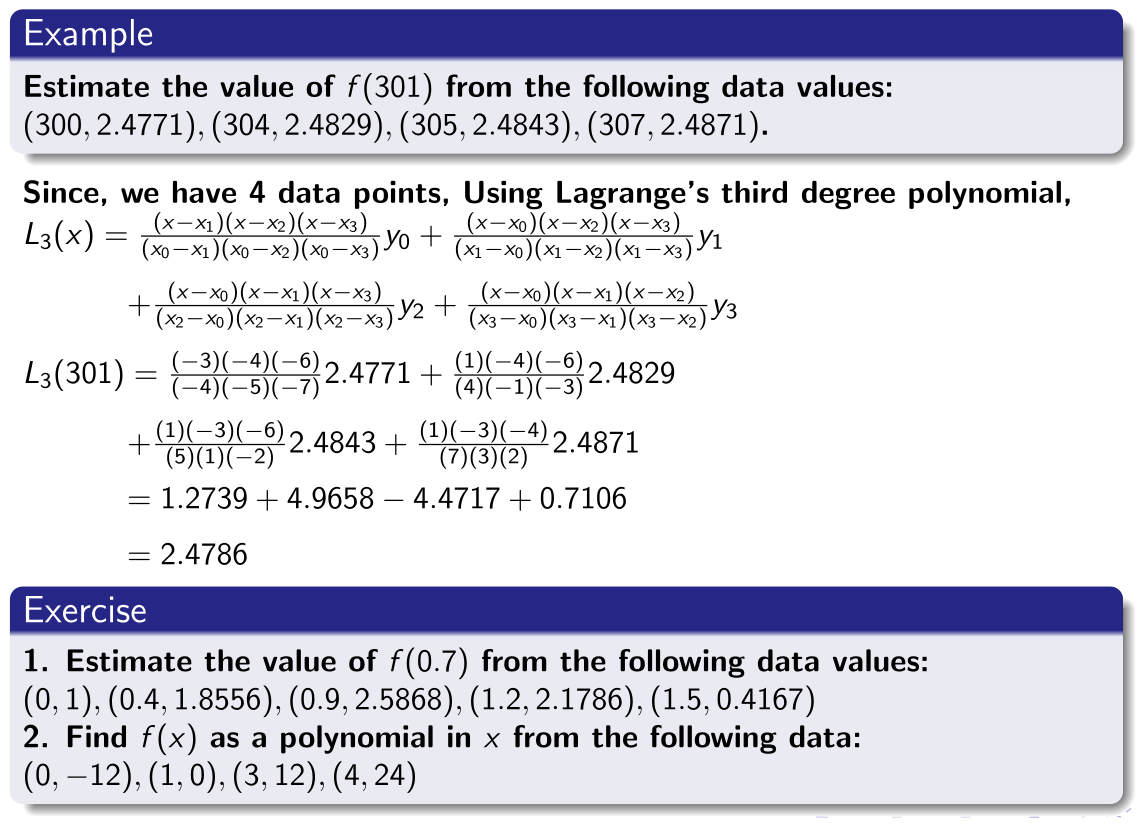
\includegraphics[width=13cm, height=12cm]{lagra_ex.png}
\end{figure}
\subsection{Disadvantage of Lagrange's Interpolation}
The Lagrange's Interpolation formula has the disadvantage that if another interpolation point were added, then interpolation coefficients $l_i(x)$ will have to be recomputed. We therefore see an interpolation polynomial which has the property that a polynomial of higer degree may be derived from it by simply adding new terms. Newton's general interpolation formula is one such formula.

\section{Divided Differences}
Given $(n+1)$ points, $(x_0,y_0), \, (x_1,y_1), \, ..., \, (x_n,y_n)$ of $x$ and $y(x)$, with $x$ values equally spaced, the divided differences of order $1,2,...,n$ are defined by the relations:
\begin{align*}
  [x_0,x_1] &= \frac{y_1 - y_0}{x_1 - x_0} \\[1mm]
  [x_0,x_1,x_2] &= \frac{[x_1, x_2]-[x_0,x_1]}{x_2 - x_0} \\[1mm]
  ... \\
  [x_0,x_1,x_2,...,x_n] &= \frac{[x_1, x_2,...,x_n]-[x_0,x_1,...,x_{n-1}]}{x_n - x_0}
\end{align*}
It is easy to see that, $\displaystyle [x_0,x_1] = \frac{y_1 - y_0}{x_1 - x_0} = \frac{y_0}{x_0 - x_1} + \frac{y_1}{x_1 - x_0} = [x_1,x_0]$.
Again,
\begin{align*}
  [x_0,x_1,x_2] &= \frac{[x_2, x_0]-[x_0,x_1]}{x_2 - x_0} \\[1mm]
                &= \frac{1}{x_2 - x_0} \left [ \frac{y_2- y_1}{x_2 - x_1} - \frac{y_1 - y_0}{x_1 - x_0} \right ] \\[1mm]
                  &= \frac{1}{x_2 - x_0} \left [ \frac{y_2}{x_2 - x_1} -y_1 \left ( \frac{1}{x_2-x_1} + \frac{1}{x_1 - x_0} \right ) + \frac{y_0}{x_1 - x_0} \right ] \\[1mm]
  &= \frac{y_0}{(x_0-x_1)(x_0-x_2)} + \frac{y_1}{(x_1-x_0)(x_1-x_2)} + \frac{y_2}{(x_2-x_0)(x_2-x_1)}
\end{align*}
\begin{figure}[h]
  \centering
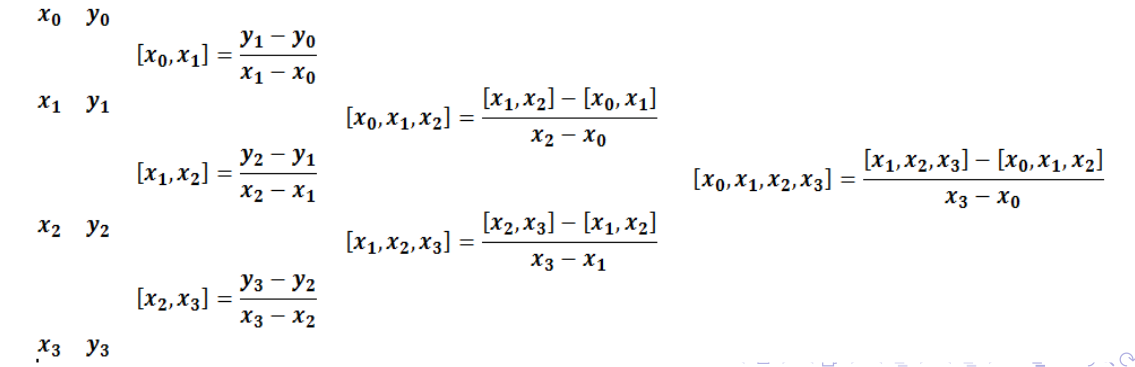
\includegraphics[width=13cm, height=5cm]{divided_for.png}
\end{figure}
\subsection{Newton's General Interpolation Formula}
We have,  $\displaystyle [x,x_0] = \frac{y - y_0}{x - x_0} \implies y = y_0 + (x-x_0)[x,x_0]$ \\[1mm]
And $\displaystyle [x,x_0,x_1] =  \frac{[x, x_0]-[x_0,x_1]}{x - x_1} \implies = [x,x_0] = [x_0,x_1] + (x-x_1)[x,x_0,x_1]$ \\[1mm]
From these two relations we get,
\begin{equation}
  \label{ninter}
  y = y_0 + (x-x_0)[x_0,x_1] + (x-x_0)(x-x_1)[x,x_0,x_1]
\end{equation}
Similarly we can get $[x,x_0,x_1] =  [x_0,x_1,x_2] + (x-x_2)[x,x_0,x_1,x_2]$ and so on...
Proceeding this way we get,
\begin{equation}
  \label{eq:ngeneral}
  \begin{gathered}
    y = y_0 + (x-x_0)[x_0,x_1] + (x-x_0)(x-x_1)[x_0,x_1,x_2] + \\[1mm]
    (x-x_0)(x-x_1)(x-x_2)[x_0,x_1,x_2,x_3] + ... \\[1mm]
    + (x-x_0)(x-x_1)(x-x_2)...(x-x_n)[x,x_0,x_1,...,x_n]
  \end{gathered}
  \end{equation}
  This Equation~\ref{eq:ngeneral} is called the Newton's general interpolation formula with divided differences.

  \begin{figure}[h!]
  \centering
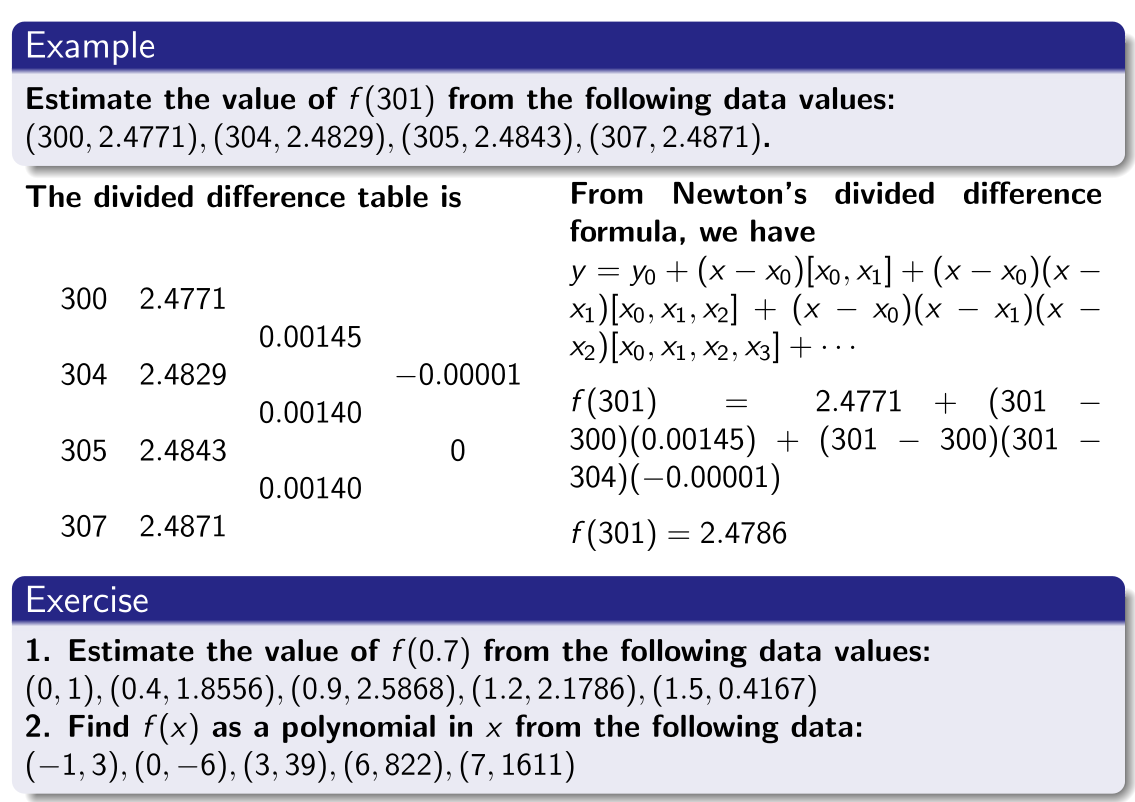
\includegraphics[width=13cm, height=11cm]{divided.png}
\end{figure}

  \section{Inverse Interpolation}
  Given a set of values of $x$ and $y$, the process of finding the value of $x$ for a certain value of $y$ is called inverse inerpolation.
  \begin{itemize}
  \item When the values of $x$ are at unequal intervals, the most obvious way of performing this process is by interchanging $x$ and $y$ in Lagrange's method.
    \item When the values of $x$ are equally spaced, the method of successive approximations on Newton's method should be used.
  \end{itemize}
\end{document}

%%% Local Variables:
%%% mode: LaTeX
%%% TeX-master: t
%%% End:
